\begin{frame}{other unfairness}
    \begin{itemize}
    \item lower round-trip gets more bandwidth
    \item can also get more bandwidth by\ldots
    \vspace{.5cm}
    \item using more connections (`independent' windows)
    \item adding more than + 1 packet to window size/RTT
    \end{itemize}
\end{frame}

\begin{frame}{alternate congestion control}
    \begin{itemize}
    \item lots of changes to congestion control
        \begin{itemize}
        \item some used in modern TCP implementations
        \end{itemize}
    \vspace{.5cm}
    \item on Internet, need to be compatible with ``normal'' TCP
    \item ``TCP-friendly''
        \begin{itemize}
        \item should not make TCP used alongside them behave poorly
        \end{itemize}
    \end{itemize}
\end{frame}

\begin{frame}{examples: checking versus TCP}
\begin{tikzpicture}
\node (a) {
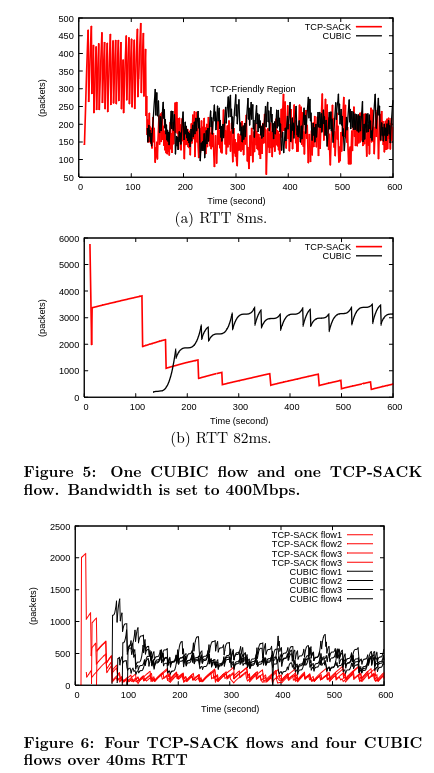
\includegraphics[height=0.9\textheight]{../congest/cubic-sack-compare}
};
\node[anchor=north west] (b) at (a.north east) {
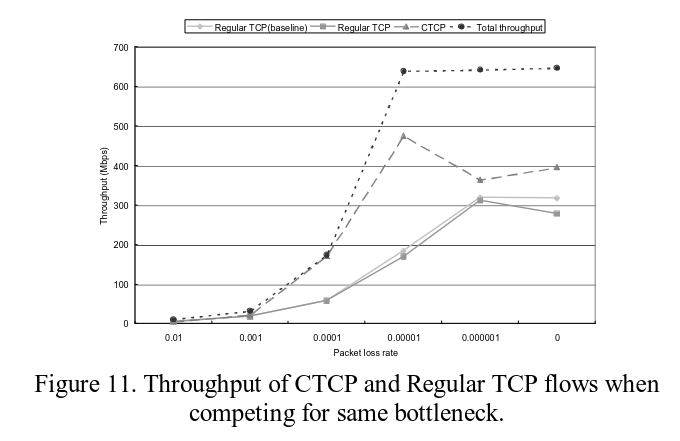
\includegraphics[height=0.6\textheight]{../congest/ctcp-regular-compare}
};
\end{tikzpicture}
\imagecredit{
from Ha, et al, ``CUBIC: A New TCP-Friendly High-Speed TCP Variant'' \\
and Tan, et al, ``A Compound TCP Approach for High-speed and Long Distance Networks''
}
\end{frame}
